\section{Predictive Modeling}

In this section we discuss the general predictive modeling process, model tuning, the problem of overfitting, and cross-validation. This draws mostly on \cite{kuhn2013applied} Chapters 2 and 4. However, I don't recommend any of the texts (APM, ESL, or ISL) for its treatment of cross-validation. Instead, consider the scikit-learn documentation (\url{https://scikit-learn.org/stable/modules/cross_validation.html}) or these lecture notes.

\subsection{Predicting $\hat{y}$}

Most of the machine learning models we will cover focus on prediction. In this world, we are not interested in marginal effects like the increase in wages attributable to schooling, standard errors, or even interpretability. Instead, we focus on some measure of predictive accuracy. A black box model is fine and a simpler model might only be preferred with parsimony as a tiebreaker.

\subsection{Tufte's Midterm Elections Model}

Let's focus on regression problems where $y$ is a continuous scalar value. For concreteness, let's say we are predicting midterm election vote share like in \cite{tufte1975determinants}. The $y$ variable is the percentage-point difference between the president's party's midterm two-party House vote share and that party's normal vote (average over the previous eight House elections).

\cite{tufte1975determinants} finds an equation 

$$\widehat{\mathrm{Vote\,Loss}} = -11.08 + 0.035\times \Delta\mathrm{Real\,Disposable\,Income} + 0.133\times \mathrm{Presidential\,Approval}.$$

This line was found based on data from 1938-1970 and the R-squared is 0.912. Recall that R-squared describes how much of the variation in $y$ is captured by the model. A perfect model gives an R-squared of 1 and a model with only an intercept equal to the average of $y$ gives an R-squared of 0. Tufte's 0.912 is impressive. With intro stats training, you might only ask for the adjusted R-squared as a follow-up. The adjusted R-squared is also impressive at 0.876.

Adjusted R-squared is a blunt way to prevent being overconfident in your model. After all, we can add new features of random noise, uncorrelated to $y$ and improve the R-squared. With enough columns, the R-squared will become exactly 1. The adjusted R-squared formula essentially penalizes the R-squared based on the number of predictor variables and the number of observations.

However, the usefulness of this as a predictive model hinges on model performance on elections \textit{after} 1970. Evaluating the model on a \textbf{test set} of previously unseen data is more data driven and it answers the question of interest more exactly. The general principle is that a model should be evaluated with new data that wasn't used in the model training. Records from 1938-1970 form the \textbf{training set} and we can assemble data from 1974-2022 as a \textbf{test set}.

Let's see how two modifications of Tufte's model holds up with test data. I was unable to replicate Tufte's Real Disposable Income variable, so I substitute a similar RDI measure using data available from the BEA. In our model 1, we include only the presidential approval variable: \code{vote_loss ~ presidential_approval}. Model 2 is spiritually the same as Tufte's though: \code{vote_loss ~ change_rdi + presidential_approval}.

We will see that none of these models performs very well on the test data.

\begin{lstlisting}[language=Python]
# hide code and output
import pandas as pd
import numpy as np
import matplotlib.pyplot as plt
import statsmodels.formula.api as smf
import statsmodels.api as sm
from predictive import calculate_out_of_sample_r2

url = 'https://raw.githubusercontent.com/alexanderthclark/pols4728/refs/heads/main/data/tufte_midterms.csv'
df = pd.read_csv(url)

# Tufte analysis
tufte_model = smf.ols(formula='vote_loss ~ pres_approval + delta_rdi', data=df[df.in_original==True]).fit()
tufte_model_sub = smf.ols(formula='vote_loss ~ pres_approval + dpi_pc_pct_yoy', data=df[df.in_original==True]).fit()
out_of_sample_average = sm.OLS(df[df.year > 1970].vote_loss, np.ones(13)).fit()
tufte_approval_only = smf.ols(formula='vote_loss ~ pres_approval', data=df[df.in_original==True]).fit()

df['single_lin_reg_residuals'] = df.vote_loss - tufte_approval_only.predict(df.pres_approval)
df['multi_reg_residuals'] = df.vote_loss - tufte_model_sub.predict(df[['pres_approval', 'dpi_pc_pct_yoy']])
df['multi_reg_predictions'] = tufte_model_sub.predict(df[['pres_approval', 'dpi_pc_pct_yoy']])

df1 = df[df.in_original==True]
df2 = df[df.year > 1970]
\end{lstlisting}

\subsubsection{Model 1}

Model 1 has an R-squared of 0.253 in the training set. From the scatter plot below, we can see that the regression line is sane but imperfect when compared to the test data. The R-squared is just 0.015 on the test set. That means using the regression model is not much better than just guessing the average from the post-1970 data.

\textit{[Note: The original notebook contains matplotlib plots. In LaTeX, these would typically be saved as separate image files and included with \textbackslash includegraphics. For brevity, I'm indicating where plots would appear.]}

\begin{figure}[H]
\centering
\textit{[Plot would show: Model 1 - Linear regression with training/test data scatter plot and residuals by year]}
\caption{Model 1: Presidential approval only. Left panel shows training data (blue) and test data (orange) with fitted regression line. Right panel shows residuals over time.}
\end{figure}

\subsubsection{Model 2}

Model 1 has an R-squared of 0.876 in the training set. From the residual scatter below, we see that the residuals become more volatile over time. Indeed, the R-squared is -0.233 (yes, negative) for the test data. That means using the regression model is worse than just guessing the average from the post-1970 data.

\begin{figure}[H]
\centering
\textit{[Plot would show: Model 2 - Predicted vs actual scatter plot and residuals by year]}
\caption{Model 2: Presidential approval and economic indicator. Left panel shows predicted vs actual values for training and test data. Right panel shows residuals becoming more volatile over time.}
\end{figure}

\subsection{Could Tufte have produced a better model?}

Above we see that model 1 is actually better than model 2 on test data. This is a case where a simple model generalizes to new data better. Should Tufte have known this? Probably not. He didn't have access to the test data. To perform model selection, he would have needed to reserve some of his eight observations for validation. With more data, we should be able to do better. The next section tries to make that process more clear.

\section{Bias-Variance Tradeoff}

There is in general a tradeoff between a model's \textit{bias} and its \textit{variance}. Bias refers to the difference between the truth and what your model predicts. Variance refers to the tendency for the exact model fit to vary according to the randomness of the data you have. Both are bad. We like unbiased models and we want low variance so that our predictions are more exact.

More complicated models tend to have higher variance. As you add more features or polynomial terms to a linear regression, your model is more sensitive to noise. However, a more simplistic model won't come as close to describing the data generating process as it really is. Thus a simple model is biased.

When we decide on a performance metric like mean squared error (MSE) we are saying that we are willing to trade a reduction in one for an increase in the other. This is somewhat different than an emphasis on unbiased models (OLS is the BLUE) you might be familiar with in other settings.

\subsection{Bias–Variance Decomposition (supervised prediction)}

\textbf{Data-generating process}
\begin{itemize}
\item $Y = \theta + \varepsilon$
\item $\mathbb{E}[\varepsilon] = 0$, $\mathbb{Var}(\varepsilon) = \sigma^2$
\item $\hat \theta$ is an estimator (random through the training sample/algorithm)
\end{itemize}

Define the test MSE:

$$\mathrm{MSE} \;=\; \mathbb{E}\!\left[(Y - \hat \theta)^2\right].$$

Substitute $Y=\theta+\varepsilon$:

$$\begin{aligned}
\mathrm{MSE}
&= \mathbb{E}\!\left[(\theta+\varepsilon-\hat \theta)^2\right] \\
&= \mathbb{E}\!\left[(\theta-\hat \theta)^2\right] + \mathbb{E}[\varepsilon^2] + 2\,\mathbb{E}\!\left[\varepsilon\left(\theta-\hat \theta\right)\right).
\end{aligned}$$

Because $\mathbb{E}[\varepsilon]=0$ and the noise $\varepsilon$ is independent of the training randomness in $\hat \theta$, the cross term is $0$. Hence

$$\mathrm{MSE} \;=\; \underbrace{\mathbb{E}\!\left[(\theta-\hat \theta)^2\right]}_{\text{estimation error}}
\;+\; \underbrace{\sigma^2}_{\text{irreducible noise}}.$$

Now split the estimation error into $\mathrm{bias}^2$ and variance:

$$\begin{aligned}
\mathbb{E}\!\left[(\theta-\hat \theta)^2\right]
&= \mathbb{E}\!\left[(\hat \theta-\mathbb{E}[\hat \theta] + \mathbb{E}[\hat \theta]-\theta)^2\right] \\
&= \mathbb{E}\!\left[(\hat \theta-\mathbb{E}[\hat \theta])^2\right] + (\mathbb{E}[\hat \theta]-\theta)^2 + 2\,\mathbb{E}\!\left[(\hat \theta-\mathbb{E}[\hat \theta])(\mathbb{E}[\hat \theta]-\theta)\right] \\
\end{aligned}$$

The first term is the variance of $\hat{\theta}$ by definition. The second term is the squared bias, by definition. The last, cross term is zero (the second factor is constant with respect to the expectation over training randomness), so

$$\begin{aligned}
\mathbb{E}\!\left[(\theta-\hat \theta)^2\right] &= \underbrace{\mathbb{Var}(\hat \theta)}_{\text{variance}} + \underbrace{(\mathbb{E}[\hat \theta]-\theta)^2}_{\text{bias}^2},
\end{aligned}$$

Therefore,

$$\boxed{\ \mathrm{MSE} = \underbrace{(\mathbb{E}[\hat \theta]-\theta)^2}_{\text{bias}^2} + \underbrace{\mathbb{Var}(\hat \theta)}_{\text{variance}} + \underbrace{\sigma^2}_{\text{irreducible noise}}\ }.$$

\subsubsection{Interpretation}

\begin{itemize}
\item \textbf{Bias}: systematic error from model misspecification/rigidity.
\item \textbf{Variance}: sensitivity to the particular training sample.
\item \textbf{Noise}: randomness you cannot remove.
\end{itemize}

Making the model more flexible typically reduces bias but increases variance restricting it does the opposite. Optimal predictive performance sits where $\mathrm{bias}^2$ + variance is minimized.

\subsubsection{Examples}

Let $f(x) = \sin x + \varepsilon$, where $\varepsilon$ is normally distributed, iid noise. Suppose we observe $x$ drawn uniformly from $[0,\pi]$ so we only have the symmetric inverted-U shape.

\begin{figure}[H]
\centering
\textit{[Plot would show: Three panels showing sine function with different datasets and linear vs quadratic fits]}
\caption{Sine function examples showing bias-variance tradeoff between linear and quadratic models on different training datasets.}
\end{figure}

In the above, the simpler model will perform much better if the distribution of $x$ values shifts (technically called covariate shift), so that we start observing values $x>\pi$. The more complex, quadratic model is probably better in all other circumstances.

Sometimes the simpler model is better for any sample of $x$ values from the same distribution. This is a more pure bias variance tradeoff. Suppose instead the actual data generating process is one of pure noise $g(x) = \varepsilon$, but that there is a lot of noise so the standard deviation of the noise is high. The quadratic model is \textit{correctly specified} but, because it is so sensitive to the noise, it might not perform as well as the biased linear model with lower variance. Hence the tradeoff.

\begin{figure}[H]
\centering
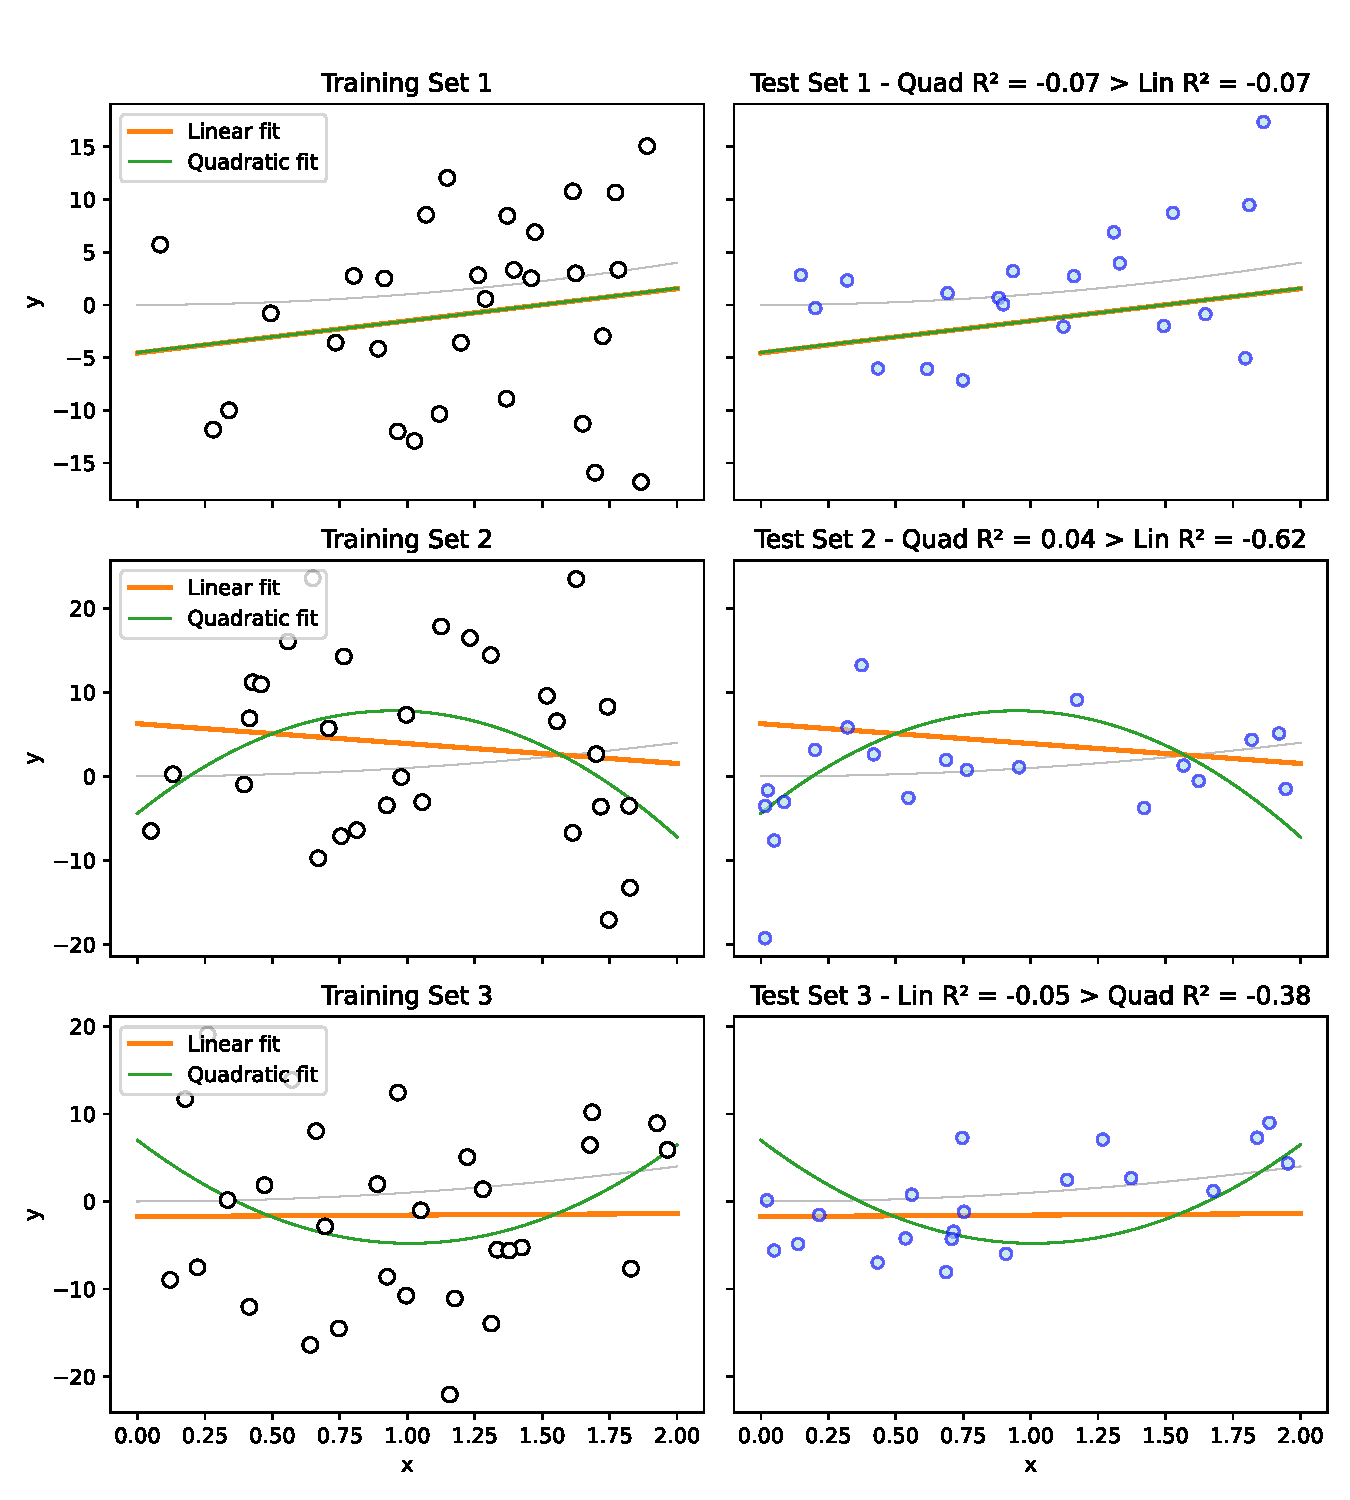
\includegraphics[width=\textwidth]{images/scatter_bias_variance.pdf}
\caption{Quadratic truth with noise showing training vs test performance for linear and quadratic models.}
\label{fig:bias-variance}
\end{figure}

\section{Validation and Model Selection}

We have seen how simple, biased models can sometimes generalize better than unbiased models. We have seen that complex models will fit our training data better but fail to perform well on test data. We have even critiqued Ed Tufte with the benefit of hindsight. Soon, it will be our turn to step into the arena and create our own models. Given that our goal is to produce a model that performs well on new data, we need to do our own validation that this will be the case. The way this is typically done is by \textbf{cross validation}. Cross validation has two uses:

\begin{enumerate}
\item Obtain a measure of the performance of your model
\item Tune your model's \textbf{hyperparameters}. This is called model selection.
\end{enumerate}

Hyperparameters are model parameters that need to be set by the researcher. Neural networks and other complex models involve many hyperparameters. If you are working with a fixed OLS specification, then there are no hyperparameters. The slope of a regression line is \textit{not} a hyperparameter, because it is determined by the model training process. However, we might consider the degree of polynomial that we use in a regression to be a hyperparameter.

\subsection{Simple Holdout Validation}

The most basic form of validation goes like this: randomly split the data into training, test, and a \textit{validation} (aka \textit{dev}) set. Then

\begin{enumerate}
\item Train each model variant (eg different polynomial specifications) on the training set.
\item Measure the error on the dev set.
\item Pick model with the lowest error on the the dev set.
\item Reserve the test set to get a final measure of the model performance.
\end{enumerate}

One rule of thumb is to use 60\% of your data for training, 20\% for dev, and 20\% for test. With large data, you might keep more data for training. Large is relative to the size of an effect you're trying to detect, so we won't make this more precise for now.

This method enables us to perform model selection and to get an estimate of our model's error. You might find it striking that we \textit{make no decisions on the basis of the test set}. When data is scarce, this is obviously inconvenient. Why can't we use the dev set error to report on our model? Each measurement is a noisy read on the actual model performance. Once we select the model that looks the best on the dev set, we create some bias--we're selecting for models that perform very well by chance. Of course, we still want to select the model with the best performance, but we shouldn't be surprised if the model doesn't do quite as well on the test set. This phenomenon is sometimes referred to as \textit{model-selection bias}, an instance of the \textit{winner's curse}, or simply \textit{optimistic bias}.

Whenever you select for an extreme, you tend to end up capturing what might be some exceptional noise. As an analogy, consider all of the Forbes 30 Under 30 honorees who have gone to jail. By selecting for success, as it is noisily measured, Forbes ends up honoring a few people who are fraudsters or just very lucky (see Twyman's Law and regression to the mean).

\subsection{Cross Validation (For Model Performance)}

With scarce data and enough computing power, cross validation is often preferred, where we rotate the data through training and validation sets. Specifically in $\mathbf{k}$-\textbf{fold} validation,

\begin{enumerate}
\item Randomly split the data in $k$ partitions, or folds, of equal size.
\item Choose $k-1$ folds for training.
\item Use the remaining fold for validation--for a measure of performance.
\item Repeat 2-3 so that each fold is used as a validation set.
\item Compute the cross-validation estimate as the size-weighted mean of the fold-level validation errors. If folds are equal size, this reduces to the simple average.
   $$\widehat{\mathrm{CV}}=\sum_{k=1}^K \frac{n_k}{N}\,\mathrm{Err}_k.$$
\end{enumerate}

There is a sort of bias variance tradeoff in choosing $k$. If $k$ is small, your final performance estimate is pessimistic because the model is trained on relatively few data points. If $k$ is large (for instance, in the extreme of $k=n$, leave-one-out cross validation), then there is less bias but higher variance. $k$ between 5 and 10 is usually recommended.
   
This will generally give you a good measure of your model's performance on new data \textit{as long as you aren't using this for model selection.} \cite{varma2006bias} shows cross validation is biased in this case, though this isn't made especially clear in ESL and other texts.

\subsection{Nested Cross Validation (For Model Selection and Model Performance)}

In nested cross validation, we use two layers of cross validation: an inner loop for model selection (hyperparameter tuning) and an outer loop for performance estimation. This approach provides an unbiased estimate of model performance while avoiding the model-selection bias discussed previously.

The process works as follows:

\begin{enumerate}
\item \textbf{Outer Loop} (Performance Estimation):
   \begin{itemize}
   \item Split data into $K_{\mathrm{outer}}$ folds
   \item For each outer fold $k = 1, ..., K_{\mathrm{outer}}$:
     \begin{itemize}
     \item Hold out fold $k$ as the test set
     \item Use the remaining $K_{\mathrm{outer}} - 1$ folds for the inner loop
     \end{itemize}
   \end{itemize}

\item \textbf{Inner Loop} (Model Selection):
   \begin{itemize}
   \item Split the training data (from outer loop) into $K_{\mathrm{inner}}$ folds
   \item For each hyperparameter configuration:
     \begin{itemize}
     \item Perform $K_{\mathrm{inner}}$-fold cross validation
     \item Calculate average validation performance
     \end{itemize}
   \item Select the best hyperparameter configuration
   \item Retrain model with best hyperparameters on all inner loop data
   \end{itemize}

\item \textbf{Evaluation}:
   \begin{itemize}
   \item Test the model from step 2 on the held-out outer fold
   \item Repeat for all outer folds
   \item Report the average performance across all outer folds as the final estimate
   \end{itemize}
\end{enumerate}

Note, your average performance measure might average over models with different hyperparameter and can only be interpreted as the performance of your general algorithm.

In my experience in industry, a degenerate case of nested cross validation is the most common. $K_{\mathrm{outer}}$ is usually set to one, so this is just cross-validation over a training+dev set and with a test set that is left untouched until after you have selected your model. This also makes it easier to decide what hyperparameters you should actually pick if you're deploying a model.

\subsubsection{Why Nested Cross Validation?}

Using regular cross validation for both model selection and performance estimation leads to optimistic bias. When you select the best-performing model based on cross validation scores, you're essentially ``peeking'' at the test data through the selection process. The model that performs best might have gotten lucky with the particular data splits.

Nested cross validation separates these concerns:
\begin{itemize}
\item The inner loop finds the best hyperparameters for each outer training set
\item The outer loop provides an unbiased estimate of how well this model selection procedure works on truly unseen data
\end{itemize}

\subsection{Time Series, Unbalanced Data, and Other Complications}

For time series, the use of longitudinal holdouts are essential so that your validation and test sets contains data from a later time period than the data used for training.

\section{Summary}

We've now learned about the predictive modeling process. Model tuning and selection is prone to the problem of over-fitting. Performance measures like R-squared (and adjusted R-squared) are misleading when calculated based on training data. A model's performance can only truly be measured by using completely new test data that was not involved in the training process. The researcher needs to remain disciplined and use procedures like cross-validation to make model selection more systematic, transparent, and reliable. As noted by Susan Athey (\url{https://www.econtalk.org/susan-athey-on-machine-learning-big-data-and-causation/}), instead of researchers subjectively choosing variables and testing specifications behind the scenes, we can now explicitly use data to determine which variables matter. This technological shift enables what \cite{grimmer2021machine} describe as a move away from purely deductive social science toward a more inductive, iterative approach where researchers can discover patterns in data rather than only testing pre-specified hypotheses.

\section{Exercises}

\begin{tcolorbox}[breakable, size=fbox, boxrule=1pt, pad at break*=1mm,colback=cellbackground, colframe=cellborder, title=Exercise: Tufte Model Comparison]
Using \code{tufte_midterms.csv}, build a few models using data from 1970 and earlier. Compare the test R-squared for the different model specifications. What specification performs best?
\end{tcolorbox}

\begin{tcolorbox}[breakable, size=fbox, boxrule=1pt, pad at break*=1mm,colback=cellbackground, colframe=cellborder, title=Exercise: Cross-Validation Usage]
Lisa and Bart are trying to find the best model to predict the quantities of oil underground. Lisa chooses her model by (1) dividing her data into test and training. (2) She compares the performance of several different models and hyperparameter settings using 5-fold cross validation on the the training set. Each model is trained five times and evaluated on the five different holdout folds. She obtains an estimate of the model performance by averaging over each of the five evaluations. (3) She picks the winning model and tuning parameters based on the CV procedure. (4) She uses the test set at the end to get a final measure of performance for the selected model.

Bart uses a similar procedure but he picks the winner by using the \textit{test} set. He uses CV to tune different types of models. Then, he compares each tuned model on the test set and picks the model with the best performance.

Who uses cross validation correctly? Lisa? Bart? Both? Neither?
\end{tcolorbox}

\begin{tcolorbox}[breakable, size=fbox, boxrule=1pt, pad at break*=1mm,colback=cellbackground, colframe=cellborder, title=Exercise: James-Stein Estimator]
Consider the estimator: $\theta_\alpha = (1 - \alpha)Y$, where $\alpha$ is a constant in $[0,1]$ and $Y\in \mathbb{R}^3$ is vector of independent normal random variables where $Y_i\sim N(\theta_i, 1)$ for $i=1,2,3$.

1.) Show that $\mathrm{MSE}(\alpha) = \mathbb{E}_Y \Vert \theta - \theta_\alpha \Vert^2  = \alpha^2 \Vert \theta \Vert^2 + 3(1-\alpha)^2 $

2.) Find the value of $\alpha$ that minimizes the MSE.

3.) Show the MSE-optimal $\theta_\alpha$ is also biased.
\end{tcolorbox}

\begin{tcolorbox}[breakable, size=fbox, boxrule=1pt, pad at break*=1mm,colback=cellbackground, colframe=cellborder, title=Exercise: P-hacking vs Overfitting]
In what ways are p-hacking and overfitting similar? In what ways are they different?
\end{tcolorbox}